\documentclass[withoutpreface,bwprint]{cumcmthesis}%
\usepackage[T1]{fontenc}%
\usepackage[utf8]{inputenc}%
\usepackage{lmodern}%
\usepackage{textcomp}%
\usepackage{lastpage}%
\usepackage{amsmath}%
\usepackage{graphicx}%
\usepackage{amssymb}%
\usepackage{cite}%
\usepackage{hyperref}%
\usepackage{pythonhighlight}%
\usepackage{longtable}%
%
\title{数学建模}%
\bibliographystyle{plain}%
\tihao{A}%
\baominghao{0001}%
\schoolname{最强大学}%
\membera{a}%
\memberb{b}%
\memberc{c}%
\supervisor{teacher}%
\yearinput{2020}%
\monthinput{4}%
\dayinput{20}%
%
\begin{document}%
\normalsize%
\maketitle%
\begin{abstract}%

这是摘要
%
\end{abstract}%
\tableofcontents%

%
\section{符号说明}%
\label{sec:}%
\begin{longtable}{c c }%
\hline%
\hline%
符号&说明\\%
\hline%
\endhead%
\hline%
\endfoot%
\hline%
\hline%
\endlastfoot%
\end{longtable}

%
\section{问题分析}

这是问题分析:$y=x$

再打一个行间公式$y=ax^2$

行内公式
$$
y=ax^2+bx^y+cx^3
$$

还有一些问题

插入一个照片

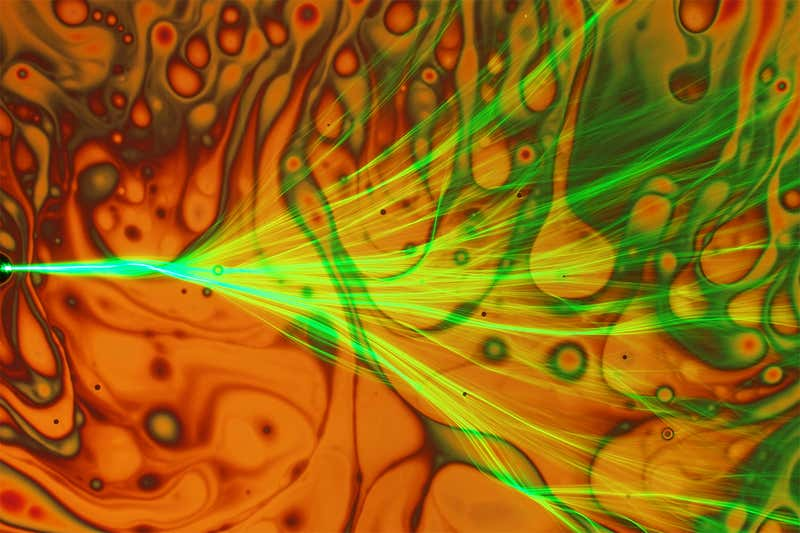
\includegraphics[None]{1.jpg}

后面补充几句话
%
\end{document}